\begin{enumerate}
	\item Avec le tarif B, le prix payé pour douze demi-journées est, en euro : \quad $15 + 3,50\times 12 = 15 + 42 = 57$.
	\item \begin{itemize}
		\item  $f(x)$ représente le tarif payé pour $x$ demi-journées avec le tarif B : $f(x) = 3,5x + 15.$

Chaque demi-journée $x$ coûte en euro, $3,50$ donc un total de $3,5x$, auxquels on ajoute l'abonnement de 15\,\euro{}.

	\item $g(x)$ représente le tarif payé pour $x$ demi-journées avec le tarif C: $g(x) = 64$.

Le tarif est constant, égal à 64\,\euro{}, quel que soit le nombre de demi-journées..

	\item $h(x)$ représente le tarif payé pour $x$ demi-journées avec le tarif A: $h(x)=5,5x$.

Chaque demi-journée $x$ coûte en $5,50\,\euro$ donc un total de $(5,5x)$\,\euro{} pour $x$ demi-journées.
	\end{itemize}


	\item \begin{itemize}
		\item  $d_1$ est une droite dont l'ordonnée à l'origine est 15, donc est la représentation graphique de la fonction affine $f$.
		\item $d_2$ est parallèle à l'axe des abscisses, donc représente la fonction constante $g$.
		\item $d_3$ est une droite contenant l'origine ; elle représente la fonction linéaire $h$.
	\end{itemize}
	\item La droite ($d_1$) ne représente pas une situation de proportionnalité, puisque la fonction associée n'est pas linéaire. Graphiquement, la droite ne passe pas par l'origine du repère. $(f(0) \ne 0)$.
	\item On cherche à quel moment le tarif B, représenté par des points de la droite $(d_1)$ devient plus avantageux que le tarif A (représenté par des points de la droite $(d_3)$).

Plus avantageux, cela veut dire que cela coûte moins cher, pour le même nombre de demi-journées. On cherche donc à partir de quel antécédent les points de la droite $(d_1)$ sont  en-dessous des points de  la droite $(d_3)$.

C'est à partir de 8 demi-journées que le tarif B est plus avantageux.

\emph{Vérification} :

$\bullet~$ $f(7 ) = 3,5 \times 7 + 15 = 24,5 + 15 = 39,50$ et $h(7) = 5,5 \times 7 = 38,50$ , donc $f(7) > h(7)$ :

$\bullet~$ $f(8 ) = 3,5 \times 8 + 15 = 28 + 15 = 43$ et $h(8) = 5,5 \times 8 = 44$ , donc $f(8) < h(8)$.

	\begin{center}
		%Début Tikz
		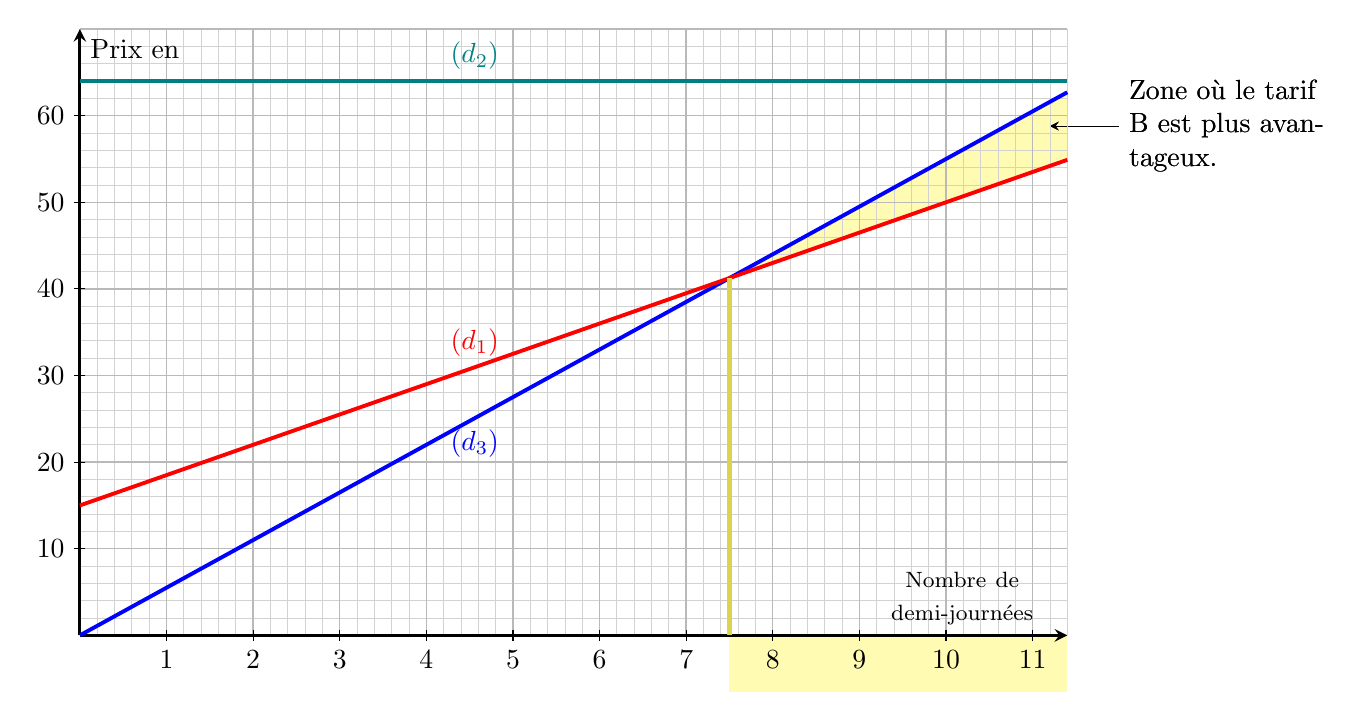
\begin{tikzpicture}[x = 11mm, y = 1.1mm, > = stealth]
			\fill[yellow!30] (7.5,41.25) --(11.4,62.7)--(11.4,54.9);
			\draw[<-] (11.2,58.8)--(12,58.8) node[right, text width=2.5cm]{Zone où le tarif B est plus avantageux.} ;
			\fill[yellow!30] (7.5,0) rectangle (11.4,-6.5);
			\draw[<-] (11.2,58.8)--(12,58.8) node[right, text width=2.5cm]{Zone où le tarif B est plus avantageux.} ;
			\draw[color  =  gray!35, line width  =  0.3pt, xstep = 0.2, ystep  =  2] (0,0) grid (11.4,70);
			\draw[color  =  gray!55, line width  =  0.5pt, xstep = 1, ystep  =  10] (0,0) grid (11.4,70);
			\draw[->,line width = 1pt] (0,0) -- (11.4,0) node[above left,text width = 2.4cm,align  =  center] {\footnotesize Nombre de demi-journées};
			\draw[->,line width = 1pt] (0,0) -- (0,70) node[below right] {Prix en \euro{}};
			\foreach \x in {1,...,11}
			\draw (\x,2pt) -- (\x,-2pt) node[below] {\np{\x}};
			\foreach \y in {10,20,...,60}
			\draw (2pt,\y) -- (-2pt,\y) node[left] {\np{\y}};
			\draw[teal,line width = 1.4pt] (0,64) -- (11.4,64) node[pos = 0.4,above]{$(d_2)$};
			\draw[blue,line width = 1.4pt] (0,0) -- (11.4,62.7) node[pos = 0.4,below]{$(d_3)$};
			\draw[red,line width = 1.4pt] (0,15) -- (11.4,54.9)
			node[pos = 0.4,above]{$(d_1)$};
			\draw[black!20!yellow!80, line width=2pt] (7.5,41.25)--(7.5,0) ;
		\end{tikzpicture}
		%Fin Tikz
		%		%Début PSTricks
		%		\psset{xunit = 1cm,yunit = 0.1cm,arrowsize = 2pt 3}
		%		\begin{pspicture}(-0.6,-5)(11,85)
			%			\psaxes[linewidth = 1.25pt,Dy = 10,labelFontSize = \scriptstyle]{->}(0,0)(0,0)(11,85)
			%			\multido{\n = 0+1}{12}{\psline[linewidth = 0.15pt](\n,0)(\n,85)}
			%			\multido{\n = 0+10}{9}{\psline[linewidth = 0.15pt](0,\n)(11,\n)}
			%			\psplot[plotpoints = 2000,linewidth = 1.25pt,linecolor = red]{0}{11}{3.5 x mul 15 add}
			%			\psplot[plotpoints = 2000,linewidth = 1.25pt,linecolor = blue]{0}{11}{5.5 x mul}
			%			\psline[linewidth = 1.25pt,linecolor = green](0,64)(11,64)
			%			\uput[u](9,0){\footnotesize Nombre de demi-journées}
			%			\uput[r](0,83){\footnotesize Prix en \euro}
			%			\rput(3,14){\blue $(d_3)$}\rput(3,30){\red $(d_1)$}\rput(3,66){\green $(d_2)$}
			%		\end{pspicture}
		%Fin PSTricks
	\end{center}

	\item \begin{enumerate}
		\item On veut traduire la fonction $f$ pour le tableur. \quad $f(x) = 15 + 3,5x$

		On peut procéder par élimination :
		\begin{itemize}
			\item \textsf{= 15+3,5*$x$}\quad ne convient pas, car le tableur ne connait pas $x$, il faut lui expliquer dans quelle cellule il trouvera la valeur $x$ correspondant à ce que l'on veut afficher;
			\item \textsf{= 15+3,5*1}\quad ne convient pas. Le résultat affiché dans la cellule \textsf{B3} serait correct, \textbf{mais}, on veut que la formule soit correcte \emph{étirée vers la droite}. Si on étire cette formule vers la droite, le calcul sera toujours le même, le 1 ne sera pas remplacé par 2, 3 et ainsi de suite;
			\item \textsf{= 15+3,5*B1}\quad est donc la bonne formule, par élimination, et parce que c'est bien dans la cellule \textsf{B1} que l'on va trouver l'antécédent du tarif que l'on veut calculer.
		\end{itemize}

		La formule à taper est donc :\quad\textsf{  = 15+3,5*B1.}

		\item Le tarif C devient plus avantageux à partir de la 14\up{e} demi-journée, le prix devenant supérieur ou égal à 64. (la cellule \textsf{P2} contient un nombre plus grand que 64).

Le tableur indique $64,5$ mais le résultat en euro et cent d'euro est $64,50$.

		\emph{Vérification par le calcul (non demandée) :}

$3,5x + 15 <  64$ \quad revient à \quad $3,5x<  64-15
	$ ou $3,5x <  49$ \quad donc \quad $x < \dfrac{49}{3,5}$.

Comme \quad $\dfrac{49}{3,5} = \dfrac{490}{35} = \dfrac{7\times 70}{7\times 5} = \dfrac{70}{5} = 14$, \quad on retrouve bien le résultat : à partir de 14 demi-journées.
	\end{enumerate}
\end{enumerate}
